\documentclass{beamer}


% Load essential packages
\usepackage{hyperref} % Only load once to avoid conflicts
\usepackage{stile}
\usepackage{subcaption}
\usepackage{tcolorbox}
\usepackage[font=scriptsize,skip=1pt]{caption}
\usepackage[T1]{fontenc}
\usepackage{csquotes}
\usepackage[backend=biber, style=authoryear, maxnames=3, minnames=1, abbreviate=false, date=long, url=false, isbn=false, doi=false]{biblatex}
\addbibresource{lecture8/bib.bib} % Ensure this matches your bibliography file name

\interfootnotelinepenalty=10000

\usepackage{latexsym, amsmath, xcolor, multicol, booktabs, calligra}
\usepackage{graphicx, pstricks, listings, stackengine}

% Hyperref setup
\hypersetup{
    hidelinks,
    colorlinks=true,
    linkcolor=black,
    citecolor=blue,
    urlcolor=black
}

% Font theme for Beamer
\usefonttheme[onlymath]{serif}

% Custom definitions
\def\cmd#1{\texttt{\color{red}\footnotesize $\backslash$#1}}
\def\env#1{\texttt{\color{blue}\footnotesize #1}}
\definecolor{deepblue}{rgb}{0,0,0.5}
\definecolor{deepred}{rgb}{0.6,0,0}
\definecolor{deepgreen}{rgb}{0,0.5,0}
\definecolor{halfgray}{gray}{0.55}

% Beamer color settings
\setbeamercolor{block title}{bg=blue!70!white, fg=white}
\setbeamercolor{block body}{bg=blue!10!halfgray, fg=white}
\setbeamercolor{section in head/foot}{fg=white}
\setbeamercolor{subsection in head/foot}{fg=white}
\setbeamercolor{title in head/foot}{fg=white}


% Listings settings for code highlighting
\lstset{
    basicstyle=\ttfamily\small,
    keywordstyle=\bfseries\color{deepblue},
    emphstyle=\ttfamily\color{deepred},
    stringstyle=\color{deepgreen},
    numbers=left,
    numberstyle=\small\color{halfgray},
    rulesepcolor=\color{red!20!green!20!blue!20},
    frame=shadowbox,
}

% Title page info
\author{Freya Rubel}
\title{Trade, Migration and Global Challenges}
\subtitle{The Impact of Migration on Host and Origin Countries}
\institute{}
\date{18.12.2025}

\graphicspath{{lecture8/}}

\begin{document}

\begin{frame}
    \titlepage
\end{frame}

\begin{frame}
    \tableofcontents[sectionstyle=show, subsectionstyle=show/shaded/hide, subsubsectionstyle=show/shaded/hide]
\end{frame}

\section{Dimensions of Impact}

\begin{frame}{How does Migration affect Society and Economy?}
\begin{center}
\large
    On which dimensions do you think migration can affect the country of origin and the destination country?
\end{center}
\end{frame}

\begin{frame}{Labor Market}
    \textbf{Host}
\begin{itemize}
    \item More (potential) workers, competition for work $\implies$ lower wages?
    \item Larger laborforce $\implies$ higher output/growing economy?
    % Each host country has a distinct demand for labor. Is the country relying mainly on services or not? Do the two educational system in the two countries align, which makes the translation and traning of foreign experience and qualifications easy 
\end{itemize}
    \textbf{Origin}
    \begin{itemize}
        \item Less workers $\implies$ Shrinking economy?
        \item Selective migration? $\implies$ Brain drain? % What was the reason for migration? Was it a humanitarian crisis? Was it due to economic incentives? Richer and better qualified workers are always more likely to find work someplace, which makes their bundaries to migrate lower 
        \item Labor scarcity $\implies$ rise in wages? % think about dynamic effects! if labor force is shrinking considerably or the economy is losing its most productive workers, this hurts the economy, decreases demand and thereby also decreases demand for labor, which is lowering wages again
    \end{itemize}
\end{frame}

\begin{frame}{Housing Market}
        \textbf{Host}
\begin{itemize}
    \item Scarcity in housing $\implies$ higher rents?
    \item More demand for housing $\implies$ higher activity of the building sector?
    \item Regional differences (rural vs. urban) % again depends on the type of migration we see, humanitarian migration, refugees and alysum seekers are provided for by the state, which usually tries to allocate them across the country. Economic migrants are usually seeking higher paying occupation and seek to live in cities, which are more culturally diverse and more attractive to foreigners 
\end{itemize}
    \textbf{Origin}
    \begin{itemize}
        \item Less demand for housing $\implies$ lower activity of the building sector?
        \item Opening up of housing $\implies$ lower rents?
    \end{itemize}
\end{frame}

\begin{frame}{Financial Flows}
            \textbf{Host}
\begin{itemize}
    \item Frictions in the integration of migrants into the labor force are expected to increase the demand for social spending in the short-run.
    \item For refugees and asylum seekers, international organization or cooperation (EU) can provide financial assistance for the reception and integration of migrants.
\end{itemize}
    \textbf{Origin}
    \begin{itemize}
        \item Increase in remittances $\implies$ Where does this money go?
        \item FDI from host country is likely to be directed towards migrants' origin country. 
    \end{itemize}
\end{frame}

\begin{frame}{Demography}
                \textbf{Host}
\begin{itemize}
    \item Population growth both in medium-run (potentially differences in fertility rates)
    \item Working-age migration can offset an aging populations $\implies$ relief for the pension system?
\end{itemize}
    \textbf{Origin}
    \begin{itemize}
        \item Population decline
        \item Loss of working-age population leads to imbalanced demography $\implies$ dangerous for social security system and economic development
    \end{itemize}
\end{frame}

\begin{frame}{Age Structure}
    \begin{figure}
        \centering
        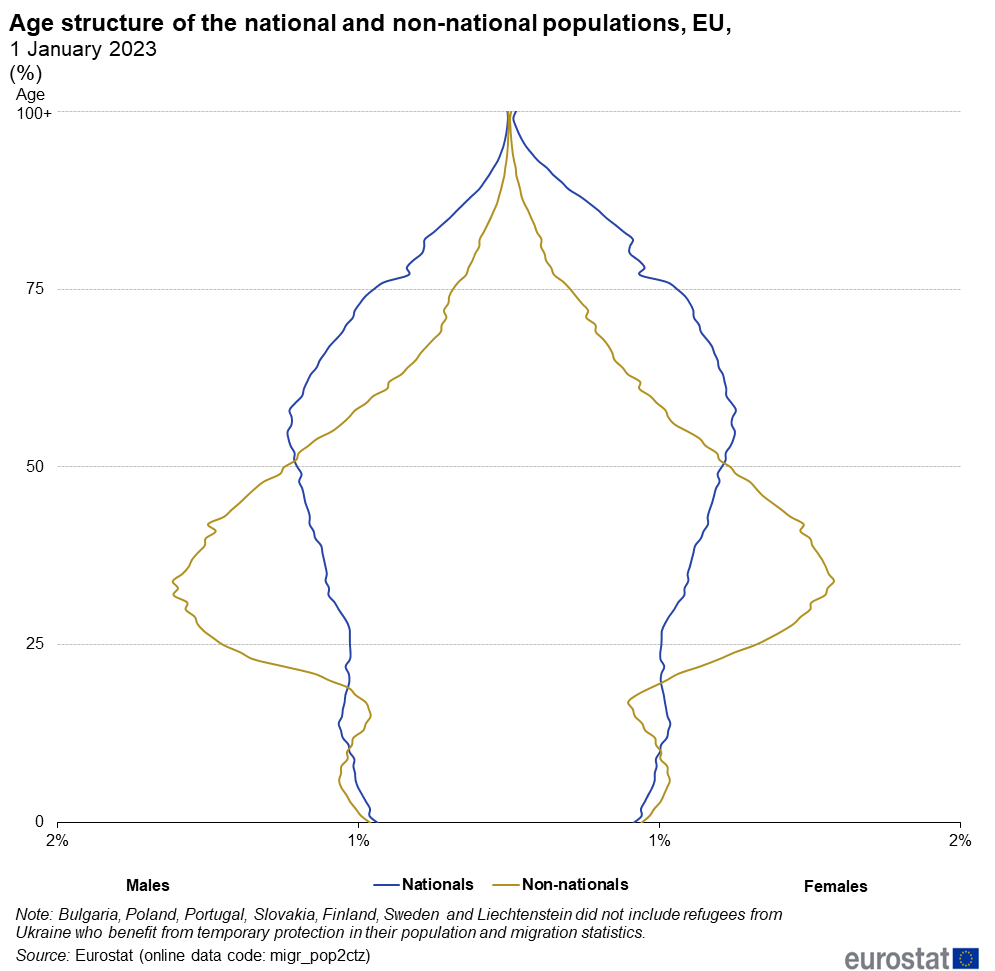
\includegraphics[width=0.69\linewidth]{Fig_8_Age_structure_of_the_national_and_non-national_populations,_EU,_1_January_2023.png}
        \label{fig:enter-label}
    \end{figure}
\end{frame}

\begin{frame}{Culture}
        \textbf{Host}
\begin{itemize}
    \item Enriched culture through new traditions, food, art, etc., 
    \item Potentially harm social cohesion and lead to tensions and defensive acts of nationalism.
\end{itemize}
    \textbf{Origin}
    \begin{itemize}
        \item Diaspora Influence: Migrants abroad can (through an information channel) shape views about the world. 
        \item Return migration may bring new ideas, values, or practices.
    \end{itemize}
\end{frame}

\begin{frame}{Politics and Institutions}
    \textbf{Host}
\begin{itemize}
    \item Immigration typically sparks new debates about immigration policies, border control, asylum, and integration.
    \item Political polarization around the topic of migration and potentially higher level of national populism.
    \item Naturalization of immigrants can change the political landscape, lead to the introduction of new parties and change the average political view of the electorate.
\end{itemize}
    \textbf{Origin}
    \begin{itemize}
        \item Bilateral Relations: Migration shapes the relations between the origin and the host countries.
        \item The information channel of diaspora citizens can change worldviews, political views, and institutions.
    \end{itemize}
\end{frame}

\section{Paper - Knowledge Spillover}

\begin{frame}{Boberg-Fazlić \& Sharp (2024)}
\begin{center}
    \begin{Large}
        Immigrant Communities and Knowledge Spillovers: Danish Americans and the Development of the Dairy Industry in the United States \\
    \end{Large}
    \begin{large}
        by Nina Boberg-Fazlić \& Paul Sharp  \\
    \end{large}
    Published in the American Economic Journal: Macroeconomics, 2024
\end{center}    
\end{frame}

\begin{frame}{Research Question \& Contribution}
\begin{tcolorbox}
    How can pre-existing immigrant communities promote economic development through knowledge spillovers?
\end{tcolorbox}
\textbf{Key Contribution:}
\begin{itemize}
    \item Examines the impact an \textit{existing} migrant community can have on technology adoption following significant developments in their country of origin
    \item Unique setting: Settlers arrived \textit{before} Denmark's dairy revolution
    \item Identifies knowledge transfer mechanism vs. skilled labor migration
\end{itemize}
\end{frame}

\begin{frame}{Literature Gap}
\textbf{What We Know:}
\begin{itemize}
    \item High-skilled immigrants promote innovation \parencite{hornung2014immigration, moser2014german}
    \item Immigration affects trade flows and long-run development \parencite{sequeira2020immigrants}
\end{itemize}

\vspace{0.3cm}
\textbf{What's Missing:}
\begin{itemize}
    \item Role of existing communities when origin country experiences breakthrough \textit{after} migration
    \item Knowledge transmission vs. human capital transfer
\end{itemize}

\vspace{0.3cm}
\textbf{This Paper:}
\begin{itemize}
    \item Natural experiment: Danish settlements pre-1880, dairy revolution 1880s
    \item Migrants couldn't have known about future technological advantages
\end{itemize}
\end{frame}

\begin{frame}{Historical Background: Denmark's Dairy Revolution}
\textbf{The Transformation (1880s-1890s):}
\begin{itemize}
    \item \textbf{Key Innovation:} Automatic cream separator (centrifuge) - 1878
    \item \textbf{Institutional Innovation:} Cooperative creameries - first in 1882
    \item \textbf{Rapid Adoption:} Hundreds of cooperatives within a decade
    \item \textbf{Market Dominance:} Captured $\sim$50\% of UK butter imports by WWI
\end{itemize}

\vspace{0.3cm}
\textbf{Productivity Gains:}
\begin{table}[h]
\centering
\small
\begin{tabular}{lcc}
\hline
Year & Danish Yields (tons/cow) & US Yields (tons/cow) \\
\hline
1860 & 1.5 & 1.2 \\
1880 & 2.5 & 1.3 \\
1900 & 2.5 & 1.5 \\
\hline
\end{tabular}
\end{table}

Denmark became world-leading, US lagged significantly behind.
\end{frame}

\begin{frame}{Danish Migration to the United States}
\textbf{Migration Characteristics:}
\begin{itemize}
    \item \textbf{Modest Scale:} Only 309,000 Danes emigrated 1840-1914 (16\% of population)
    \begin{itemize}
        \item Compare: 24\% Sweden, 39\% Norway
    \end{itemize}
    \item \textbf{Geographic Concentration:} Midwest (Iowa, Minnesota, Wisconsin)
    \item \textbf{Timing:} Small numbers pre-1880, increased from 1890s
    \item \textbf{Occupation:} Less than 1\% had dairy-related occupations
\end{itemize}

\vspace{0.3cm}
\textbf{First US Cream Separator (1883):}
\begin{itemize}
    \item Fredsville, Iowa - Danish settlement
    \item Imported from Denmark by Jeppe Slifsgaard
    \item Became "Danish Creamery" - later cooperative
\end{itemize}

\vspace{0.2cm}
\textbf{Key Point:} Pre-1880 settlements established \textit{before} Denmark's advantages emerged.
\end{frame}

\begin{frame}{Data Sources}
\textbf{US Census Data:}
\begin{itemize}
    \item Full-count microdata (1880, 1900, 1910, 1920): demographics, birthplace, occupation
    \item Agricultural census (1870-1920, county-level): dairy cows, butter production, wheat, livestock
    \item Manufacturing census (1880-1920, state-level): industrial dairy workers, butter production
\end{itemize}

\vspace{0.3cm}
\textbf{Danish Emigration Archives:}
\begin{itemize}
    \item Police protocols: $\sim$330,000 emigrants (1868-1908)
    \item Information: name, birthplace, occupation, destination
    \item Return migrants: those listing US as "last place of residence"
\end{itemize}

\vspace{0.3cm}
\textbf{Additional Sources:}
\begin{itemize}
    \item Danish-language newspapers in US (knowledge transmission measure)
    \item Geographic controls: pasture suitability, elevation, market access
\end{itemize}

\vspace{0.2cm}
\textbf{Unit of Analysis:} 2,159 counties (borders adjusted to 1870)
\end{frame}

\begin{frame}{Empirical Strategy}
\textbf{Difference-in-Differences Design:}
\begin{equation*}
Y_{it} = \beta \ln(\text{Danes}_{1880,i}) \times D_{\text{post1880}} + X_i \times I_t + \mu_i + \lambda_t + \eta_{rt} + \epsilon_{it}
\end{equation*}

\begin{itemize}
    \item \textbf{Treatment:} ln(Number of Danes in county in 1880)
    \item \textbf{Cutoff:} 1880 (before Denmark's dairy revolution)
    \item \textbf{Outcomes:}
    \begin{enumerate}
        \item ln(Dairy cows) - specialization
        \item ln(Industrial dairy workers) - modernization
        \item ln(Farm butter production) - traditional methods (should $\downarrow$)
    \end{enumerate}
\end{itemize}

\textbf{Controls:} Pasture suitability, wheat suitability, elevation, ruggedness, distance to waterways; County FE, Year FE, Region×Year FE

\vspace{0.2cm}
\textbf{Identification:} Danes settled before knowing about future dairy advantages
\end{frame}

\begin{frame}{Scatterplot - Partial Correlation}
    \begin{figure}
        \centering
        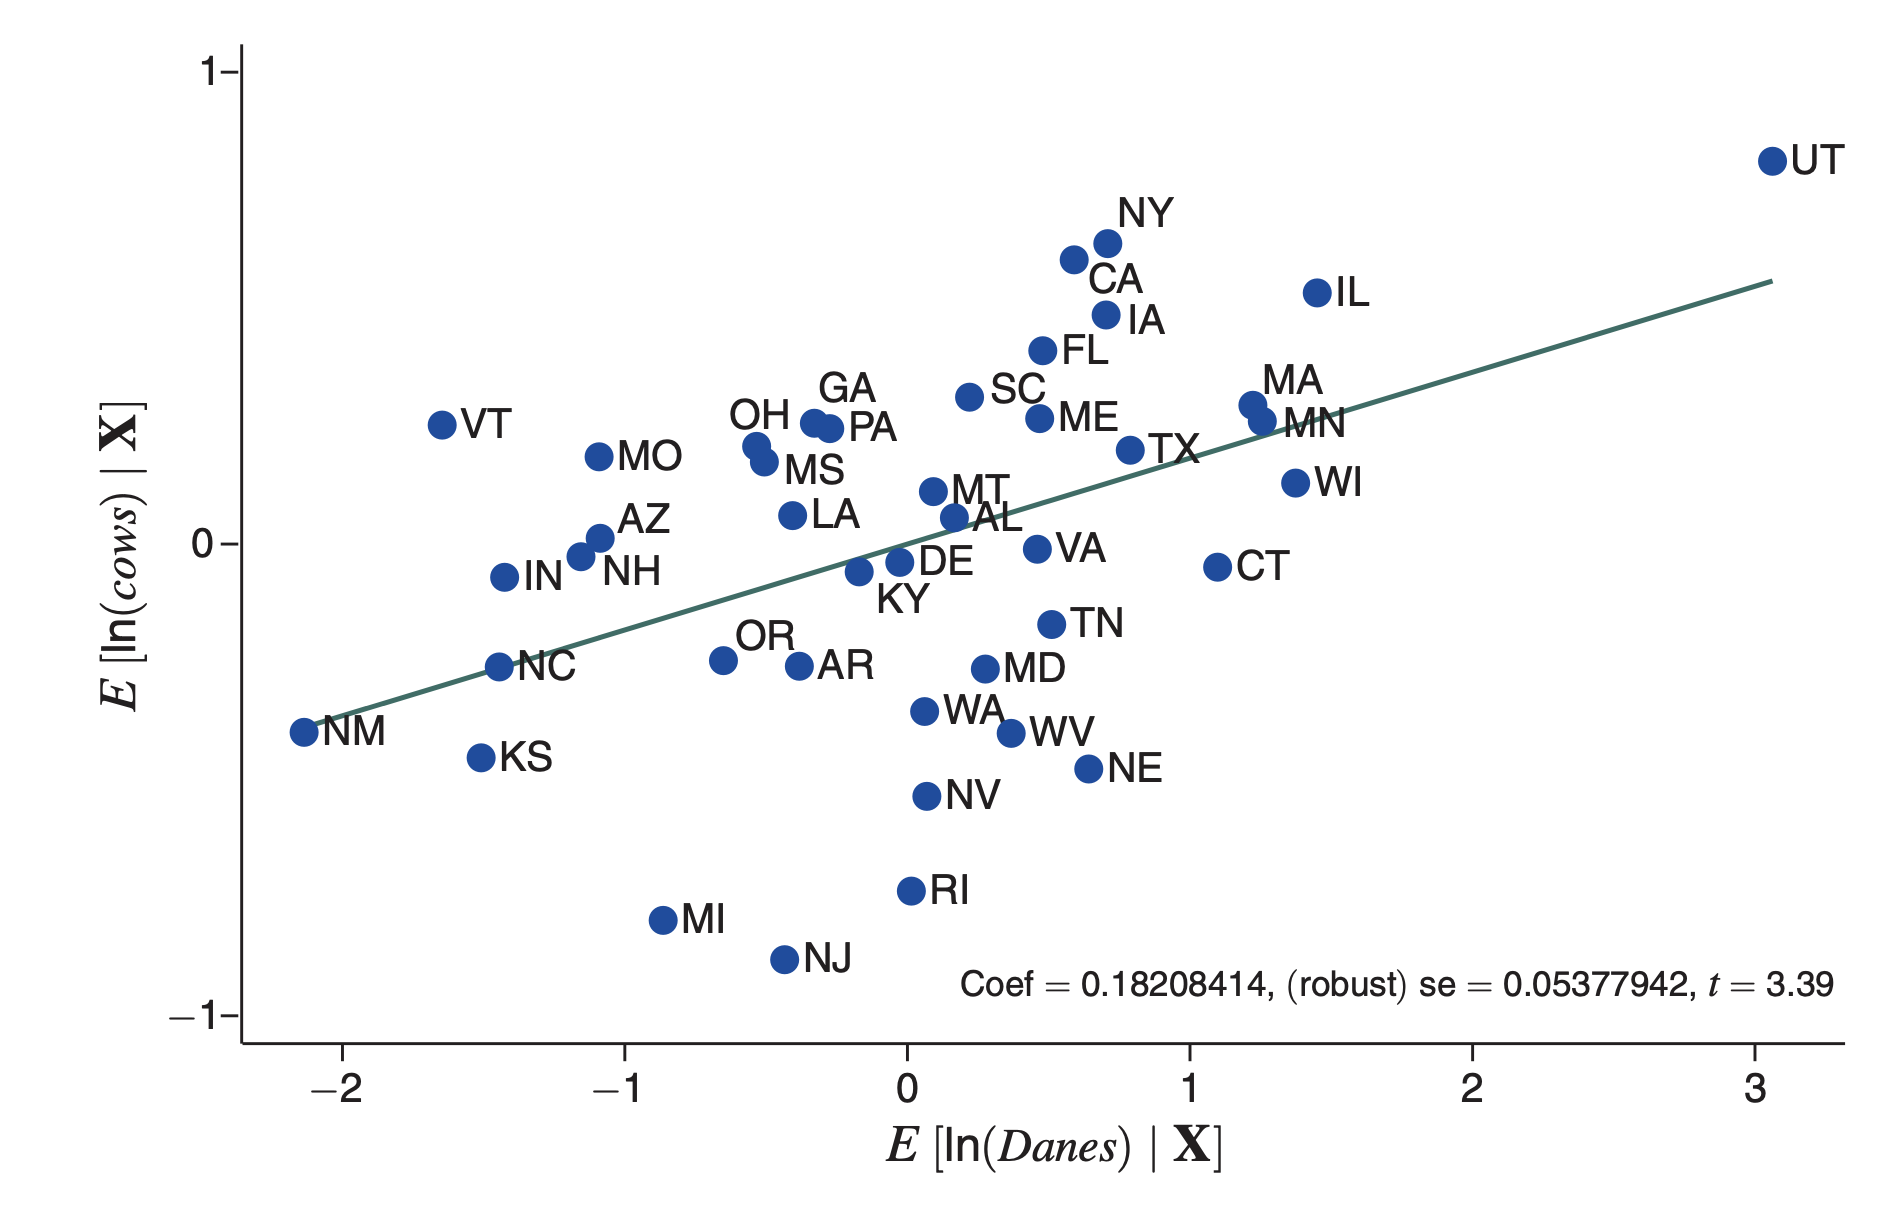
\includegraphics[width=0.75\linewidth]{Bildschirmfoto 2024-12-12 um 00.58.03.png}
        \caption{Partial Regression Plot between ln(Danes) and ln(Cows). State Level, Year 1900. Controlling for geography and region fixed effects.}
        \label{fig:scatter-cows}
    \end{figure}
\end{frame}

\begin{frame}{Main Results: Specialization \& Modernization}
\textbf{Effect on Dairy Specialization:}
\begin{itemize}
    \item \textcite{bobergfazlic2024immigrant} find that \textbf{1\% more Danes $\rightarrow$ 0.9\% more dairy cows} after 1880 ($\beta = 0.009$, SE=0.002)
    \item 1 SD increase in Danes $\rightarrow$ \textbf{4.2\% more dairy cows}
    \item Effect \textbf{persists through 1970}
\end{itemize}

\vspace{0.3cm}
\textbf{Effect on Modernization:}
\begin{itemize}
    \item \textbf{Positive effect on industrial dairy workers} ($\beta = 0.076$, SE=0.021)
    \item \textbf{Negative effect on farm butter production} ($\beta = -0.005$, SE=0.002)
    \item $\Rightarrow$ Resources shifted from traditional to modern production
\end{itemize}

\vspace{0.3cm}
\textbf{Robustness:}
\begin{itemize}
    \item No pre-trends for counties with $>$2 Danes in 1880
\end{itemize}
\end{frame}

\begin{frame}{Mechanism: Knowledge Transfer vs. People Transfer}
\textbf{Two Possible Channels:}
\begin{enumerate}
    \item Direct immigration of skilled dairymen
    \item Knowledge transfer through existing communities
\end{enumerate}

\vspace{0.3cm}
\textbf{Evidence for Knowledge Transfer:}
\begin{table}[h]
\centering
\small
\begin{tabular}{lll}
\hline
\textbf{Mechanism} & \textbf{Measure} & \textbf{Finding} \\
\hline
Skilled migration & Dairy occupation & Only 1,621 total ($<$1\%) \\
Managers & Danish managers & 6/1,110 in 1900 \\
Information & Danish newspapers & Strong effect \\
\hline
\end{tabular}
\end{table}

\vspace{0.3cm}
\textbf{Key Finding:} Effect stems from \textit{general} Danish population, not experts
\begin{itemize}
    \item All Danes facilitated information flow from Denmark to the US
    \item Knowledge spread through Danish-language press
    \item Non-Danes learned from and imitated Danish practices
\end{itemize}
\end{frame}

\begin{frame}{Spillovers to Other Groups}
\textbf{Effect on Other Scandinavians:}
\begin{itemize}
    \item \textbf{Positive spillovers to Norwegians} ($\beta = 0.013$)
    \begin{itemize}
        \item But \textit{only in counties with Danes present}
        \item Without Danes: Norwegians have no dairy effect
    \end{itemize}
    \item \textbf{Negative effect for non-Scandinavian foreigners}
    \begin{itemize}
        \item Suggests specialization in other industries
    \end{itemize}
\end{itemize}

\vspace{0.3cm}
\textbf{Why Scandinavians?}
\begin{itemize}
    \item \textbf{Linguistic proximity} 
    \item \textbf{Cultural similarity:} Shared institutions
    \item \textbf{Geographic clustering:} 70\% overlap in settlement
\end{itemize}
\end{frame}

\begin{frame}{Policy Implications}
\textbf{Lessons for Immigration Policy:}
\begin{enumerate}
    \item \textbf{Ex Ante Assessment is Difficult}
    \begin{itemize}
        \item Danish immigrants were NOT "highly skilled" upon arrival
        \item Yet had substantial long-term economic impact
    \end{itemize}
    
    \item \textbf{Timing \& Dynamics Matter}
    \begin{itemize}
        \item Benefits can emerge decades after initial arrival
        \item Developments in origin country create unexpected advantages
    \end{itemize}
    
    \item \textbf{Network Effects Are Powerful}
    \begin{itemize}
        \item Small communities can have large spillovers
        \item Knowledge transfer doesn't require mass migration
        \item Networks facilitate adoption by native population
    \end{itemize}
\end{enumerate}

\vspace{0.3cm}
\textbf{Historical Irony:} 1921 Emergency Quota Act praised Scandinavian farmers as "some of the very best" - yet would have prevented their arrival had it existed earlier
\end{frame}

\begin{frame}{Conclusion}
\textbf{Main Findings:}
\begin{itemize}
    \item Danish settlements (pre-1880) significantly boosted US dairy development
    \item Effect through \textbf{knowledge spillovers}, not direct labor supply
    \item Impact persisted for nearly a century (through 1970)
    \item Small immigrant groups can have disproportionate economic effects
\end{itemize}

\vspace{0.3cm}
\textbf{Key Mechanisms:}
\begin{itemize}
    \item Knowledge transfer through community networks
    \item Return migration and Danish-language press
    \item Spillovers to culturally/linguistically similar groups
    \item Native population learned and imitated
\end{itemize}

\vspace{0.3cm}
\textbf{Broader Implications:}
\begin{itemize}
    \item Difficult to predict which immigrants will be "desirable"
    \item Benefits may only become apparent over long time horizons
    \item Networks matter as much as individual skills
    \item Path dependence in industrial location
\end{itemize}
\end{frame}

\section{Paper - Brain Gain Hypothesis}

\begin{frame}{Batista, Lacuesta \& Vicente (2012)}
\begin{center}
    \begin{Large}
        Testing the 'Brain Gain' Hypothesis: \\
        Micro Evidence from Cape Verde \\
    \end{Large}
    \vspace{0.3cm}
    \begin{large}
        by Catia Batista, Aitor Lacuesta \& Pedro C. Vicente  \\
    \end{large}
    \vspace{0.2cm}
    Published in the Journal of Development Economics, 2012
\end{center}    
\end{frame}

\begin{frame}{Research Question \& Contribution}
\begin{tcolorbox}
Does the \textbf{prospect of future migration} increase educational investment at home?
\end{tcolorbox}

\vspace{0.3cm}
\textbf{The Debate:}
\begin{itemize}
    \item \textbf{Brain Drain (traditional):} Educated people emigrate $\rightarrow$ Origin country loses human capital
    \item \textbf{Brain Gain (new hypothesis):} Migration possibility creates education incentive $\rightarrow$ Even non-migrants invest more $\rightarrow$ Origin gains human capital
\end{itemize}

\vspace{0.3cm}
\textbf{The Context:}
\begin{itemize}
    \item 1990-2000: 63.7\% increase in highly-skilled immigrants to OECD
    \item Some countries lose 30-80\% of educated workforce
\end{itemize}

\end{frame}

\begin{frame}{The Setting: Cape Verde}

\begin{columns}
\begin{column}{0.48\textwidth}
\textbf{Basic Facts (2003):}
\begin{itemize}
    \item Small island nation, West Africa
    \item Population: $\approx$ 500,000
    \item GDP per capita: \$5,900 (PPP)
    \item 1980-2004: 4.4\% annual growth (3rd fastest in Sub-Saharan Africa)
\end{itemize}
\end{column}

\begin{column}{0.48\textwidth}
\textbf{The Paradox:}
\begin{itemize}
    \item \textbf{Highest brain drain in Africa:} 67.5\% of university-educated Cape Verdeans live abroad
    \item \textbf{Yet:} Fast human capital \& economic growth
\end{itemize}

\vspace{0.3cm}
\textbf{Migration Facts:}
\begin{itemize}
    \item 19\% of native-born live abroad
    \item Top destinations: Portugal (55\%), US (20\%)
\end{itemize}
\end{column}
\end{columns}

\end{frame}

\begin{frame}{The Research Challenge \& Strategy}

\textbf{The Problem:}
\begin{itemize}
    \item Migration and education \textbf{simultaneously determined}
    \item Reverse causality: More educated $\rightarrow$ More likely to migrate
    \item Omitted variables: Ambition, ability affect both
    \item Can't just compare migrants vs. non-migrants
\end{itemize}

\vspace{0.3cm}
\textbf{Solution: Instrumental Variables (IV) Approach} \\
Need instrument that:
\begin{enumerate}
    \item Affects expected migration probability
    \item Doesn't directly affect education decisions
    \item Is "as good as random" (exogenous)
\end{enumerate}
\end{frame}

\begin{frame}{Data}
\textbf{Primary Data Source: Custom Household Survey (2005-06)}
\begin{itemize}
    \item 1,066 households, representative sample of the population
    \item \textbf{Full migration histories} of all family members
    \item Who migrated, where, when, for how long
    \item Educational attainment, family background, assets
    \item Supplemented with: Census data, economic conditions abroad
\end{itemize}
\end{frame}

\begin{frame}{Sample and Key Variables}

\textbf{Sample Construction:}
\begin{itemize}
    \item Individuals aged 16-30 in 2006 survey
    \item Did NOT migrate before age 16 (education completed in Cape Verde)
    \item N = 1,411 (main sample)
\end{itemize}

\vspace{0.3cm}
\textbf{How Migration Status Is Observed:}
\begin{itemize}
    \item Non-migrants: Still in Cape Verde in 2006 (interviewed directly)
    \item Migrants: Migrated after age 16, now abroad (reported by families in Cape Verde)
\end{itemize}

\vspace{0.3cm}
\textbf{Outcome Variable:}
\begin{itemize}
    \item Completed intermediate secondary education (9 years of schooling)
    \item Binary: Yes = 1, No = 0
\end{itemize}
\end{frame}

\begin{frame}{Main Instrument: Family Migration Duration}
\textbf{What is it?}
\begin{itemize}
    \item Duration (years) of \textbf{longest family migration spell} when child is age 12
\end{itemize}

\vspace{0.2cm}
\textbf{Example:}
\begin{itemize}
    \item \textbf{Child A:} Uncle migrated 1985, still abroad (20 years by 2005) 
    \item \textbf{Child B:} Cousin migrated 2000, returned after 2 years 
    \item At age 12: Child A observes successful migration $\rightarrow$ Higher probability of own migration $\rightarrow$ Invests more in education?
\end{itemize}

\vspace{0.2cm}
\textbf{Why It (Might) Work as Instrument:}
\begin{itemize}
    \item \textbf{Relevance:} Predicts both expected and actual migration
    \item \textbf{Timing:} Measured at age 12, before education decisions
\end{itemize}
\end{frame}

\begin{frame}{Regression Equation}
\textbf{The Authors' Approach - Two-Stage Least Squares:}

\textbf{First Stage:} Family migration predicts actual migration
$$\text{Migrate}_{i,16-30} = \pi_0 + \pi_1 \text{FamilyMigrationDuration}_{i,12} + \pi_2 \cdot \text{Controls}_i + u_i$$

\textbf{Second Stage:} Effect on education
$$\text{Education}_i = \beta_0 + \beta_1  \widehat{\text{Migrate}}_{i,16-30} + \beta_2 \cdot \text{Controls}_i + \varepsilon_i$$

\vspace{0.2cm}
\textbf{Authors' interpretation:} Because family migration affects expectations (which drives education), and expectations correlate with actual migration, $\beta_1$ captures the effect of expected migration probability on education.
\end{frame}


\begin{frame}{Main Results}

\textbf{Naive Comparison (OLS):}
\begin{itemize}
    \item Migrants are 15 percentage points more likely to have complete 9 years than non-migrants
    \item But this is just correlation—doesn't tell us if migration prospects \textit{cause} education
\end{itemize}

\vspace{0.4cm}

\textbf{Causal Estimate (2SLS with Family Migration Instrument):}
\begin{itemize}
    \item \textcite{batista2012testing} find that a 10 percentage point increase in migration probability causes an 11.2 percentage point increase in probability of completing 9 years
    \item This uses family migration history to isolate causal effect
\end{itemize}

\end{frame}

\begin{frame}{The Key Test: Effect for Never-Migrants}

\textbf{Critical Question:} Is this about actual migration or migration prospects?

\vspace{0.3cm}
\textbf{Test (Reduced Form):}
\begin{itemize}
    \item Take sample of non-migrants (stayed in Cape Verde through 2006)
    \item For this subsample: Does family migration history \textbf{directly} predict their education?
    \item If yes $\rightarrow$ Family migration affects education even without actual migration
\end{itemize}

\vspace{0.3cm}
\textbf{Result:} 
\begin{itemize}
    \item Reduced form coefficient: 1.004-1.252 (similar to full-sample 2SLS)
    \item Family migration history strongly predicts education even for never-migrants
\end{itemize}

\end{frame}


\begin{frame}{Honest Assessment of the Evidence}

\textbf{What We Can Conclude with Confidence:}
\begin{enumerate}
    \item \textbf{Strong correlation} between family migration and education (survives many controls)
    \item \textbf{Effect exists for never-migrants} - key evidence for brain gain mechanism
    \item \textbf{Mechanism plausible:} Consistent with theory and other empirical evidence
\end{enumerate}

\vspace{0.2cm}
\begin{alertblock}{Bottom Line}
Suggestive causal evidence for brain gain, with never-migrant analysis providing most compelling support for the mechanism
\end{alertblock}
\end{frame}

\begin{frame}{Limitations}

\begin{enumerate}
    \item \textbf{Selection Concerns:}
    \begin{itemize}
        \item Families with long migrations may be systematically different
        \item Controls may not capture all unobserved characteristics
    \end{itemize}
    
   \item \textbf{External Validity:}
\begin{itemize}
    \item Specific to Cape Verde (small, moderate emigration)
    \item May not apply to very small (excessive drain) or very large countries
\end{itemize}
    
    \item \textbf{Data Limitations:}
    \begin{itemize}
        \item Survey misses complete emigrant families
        \item Cross-sectional (one time point)
    \end{itemize}
\end{enumerate}
\end{frame}


\begin{frame}{Conclusions}

\textbf{Main Findings:}
\begin{enumerate}
    \item \textbf{Evidence for brain gain in Cape Verde}
    \begin{itemize}
        \item 10pp $\uparrow$ migration probability $\rightarrow$ $\approx$ 11pp $\uparrow$ education
        \item Effect exists even for non-migrants (option value)
     \item Among high-probability individuals: 40\% migrate, 60\% stay in Cape Verde
    \end{itemize}
    \item \textbf{Mechanism: Education incentives}
    \begin{itemize}
        \item Migration option value drives investment
        \item Consistent with theory and evidence
    \end{itemize}
\end{enumerate}

\vspace{0.3cm}
\textbf{Contribution:}
\begin{itemize}
    \item First micro-level test of brain gain hypothesis
    \item Challenges "brain drain" pessimism
    \item Shows migration can benefit both origin and destination
\end{itemize}
\end{frame}

\begin{frame}{Key Takeaway \& Discussion}

\begin{tcolorbox}[colback=blue!5!white, colframe=blue!75!black, width=0.95\textwidth]
\textbf{For countries like Cape Verde:}

Migration opportunity promotes human capital development at home.

Even 67.5\% brain drain can coexist with rapid human capital growth through \textbf{education incentive effects}.
\end{tcolorbox}


\end{frame}


\begin{frame}[allowframebreaks]{References}
    \printbibliography
\end{frame}


\end{document}

